\documentclass[12pt,fleqn]{article}\usepackage{../common}
\begin{document}
Ders 22

Muhendislerin Laplace Transformunu sevmesinin sebeplerinden biri
fonksiyonlarda kesintili / birdenbire ziplayan gecisleri (jump
discontinuities) durumlarinda bozulmadan isleyebiliyor olmasidir. 

Kesintili fonksiyonlardan biri birim adim fonksiyonudur. Fonksiyonun
kendisi tartisma yaratan bir fonksiyon aslinda, sifir noktasinda hangi
degere sahip oldugu hala kararlastirilamadi. Bazilari 0 diyor, bazilari 1
diyor, ben bu derste tanimsiz birakacagim. Yani

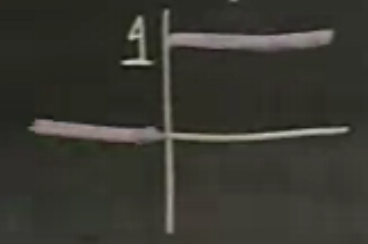
\includegraphics[height=2cm]{22_1.png}

$u(t)$ birim adim

$u(0)$ tanimsiz

Bazen sifir yerine baska bir noktada ziplama olmasini isteyebilirim. O
zaman fonksiyonu kaydirmak mumkun, mesela $a$ kadar. 

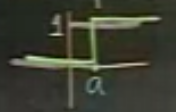
\includegraphics[height=2cm]{22_2.png}

\[ u_a(t) = u(t-a) \]

Birim Kutu

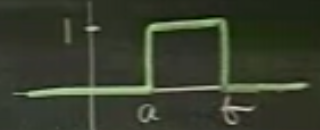
\includegraphics[height=2cm]{22_3.png}

Kutuyu birim adimlar kullanarak temsil edebilirsek iyi olur, cunku
birim adimlarin Laplace transformunu biliyoruz. 

\[ u_{ab} := u_a(t) - u_b(t) \]

\[ = u(t-a) - u(t-b) \]

Mantikli gozukuyor, $b$'ye gelene kadar birim adim gibi gidiyoruz, $b$'de
birim adimi iptal edecek sekilde birim adimi cikartiyoruz. 

Peki bu fonksiyonlar niye faydali? Diger fonksiyonlari carptiklarinda o
fonksiyonlari faydali sekillerde degistirebildikleri icin. Diyelim ki soyle
bir $f(t)$ var.

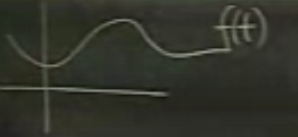
\includegraphics[height=2cm]{22_4.png}

\[ u_{ab}f(t) \]

neye benzerdi? Eger $a,b$ arasinda $u_{ab}$ 1 degerine esitse, carpim bu
aralikta $f(t)$'yi oldugu gibi alir. Diger noktalarda sifir yapar. Alttaki
sekil ortaya cikar (mavi cizgiler). 

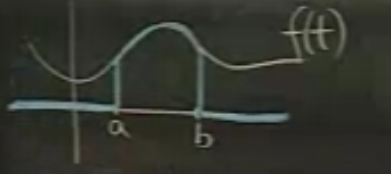
\includegraphics[height=3cm]{22_5.png}

$f(t)$'nin bir parcasini cekip cikartiyoruz yani. Bu cok ise yarayan bir
numara / teknik. 

* * *

Birim adimin Laplace Transformunu alalim.

\[ \mathcal{L}(u(t)) = \int_{0}^{\infty} e^{-st}u(t) dt  \]

Entegral alt siniri 0'dan basliyor. Birim adim 0'dan buyukse hep 1, o zaman
ustte $u(t)$'yi 1 alabiliriz. Yani ustteki aslinda 1'in Laplace
Transformudur. 

\[ = \frac{1}{s} \ \ \ s>0 
\ \ \ \label{1}
\]

Kaydirilmis birim adimin Laplace'i

\[ \mathcal{L} (u(t-a)) = 
\int_{a}^{\infty} 1 \cdot e^{-st} dt
 \]

Alt sinir $a$ oldu cunku $a$'dan once sifir, sonrasi 1. Bizi tek
ilgilendiren kisim fonksiyon 1 olduktan sonra, o zaman alt siniri 
degistiririz. 

\[ = \frac{e^{-st}}{-s} \bigg|_{a}^{\infty} =
\frac{e^{-as}}{s}
\]

Diger bir ozellik

\[ \mathcal{L}(e^{ct}f(t)) = F(s-c) \]

Ispat: Eger entegral temsilini acarsak

\[ = \int _{0}^{\infty} e^{ct}f(t)e^{-st}dt  =
\int e^{(c-s)t} f(t) dt
 \]


Bu son ifadeye baska bir yonden erisebilir miyiz? Mesela $F(s-c)$ nedir? 
$s$ yerine $s-c$ koyarsak (temel formulden turetelim)

\[ F(s-c) = \int _{0}^{\infty} f(t) e^{-(s-c)t} ft  \]

\[ = \int _{0}^{\infty} e^{(-s+c)t} dt  = \int _{0}^{\infty} e^{(c-s)t} dt   \]

Ayni ifadeye eristik. 

* * *

(1) formulundede ters yonde gidersek

\[ \mathcal{L}^{-1}(\frac{1}{s}) = ?  \]

Geriye giderken 1'e mi, birim adima mi donecegim? Simdiye kadar geriye
giderken hep 1 sectim. Artik bu yeterli degil. Problem nerede? Cunku
Laplace Transformu entegral alt siniri 0'dan basliyor, yani transform 0
oncesine bakmiyor bile. Bir fonksiyon $f(t)$ 0'dan once envai turde degere
sahip olabilir, Laplace Transformu ayni olacaktir. 

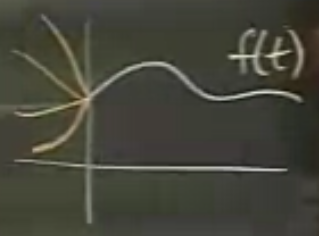
\includegraphics[height=3cm]{22_6.png}

Eger hangi tur problem ile ugrastigimizi biliyorsak bu durum bir sorun
cikarmaz. Muhendisler soyle kategorize ederler; eger bir problem simdiki
zamandan, $t=0$, baslayip ileri gidiyorsa o bir Laplace Transform
problemidir, eger gecmis zaman verisi gerekiyorsa o bir Fourier Transform
problemidir. 

Eger 1 noktasindan ( $t=0$ ) geriye giderken ortaya cikan tanimsizliktan
(ambiguity) kurtulmak istiyorsak, ters Laplace'dan elde edilen fonksiyonu
birim adim ile carpariz, boylece $t=0$ oncesi sifir olmasini garanti etmis
oluruz.

\[ f(t) \leadsto F(s) \]

\[ \mathcal{L}^{-1}(F(s)) = u(t)f(t) \]

Boylece ters Laplace ozgun (unique) hale gelir.

* * * 

Tasima (translation) ve Laplace 

$\mathcal{L}(f(t-a))$'yi $\mathcal{L}(f(t))$ temel alarak yazabilir miyiz?
Bu ne yazik ki mumkun degil. 

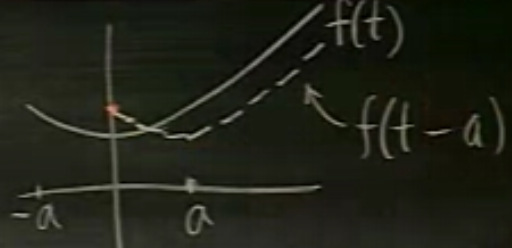
\includegraphics[height=3cm]{22_7.png}

Ustte $f(t)$'yi $a$ kadar saga kaydirdik. Kesik cizgili yeni, tasinmis
fonksiyonu niye duz cizgili fonksiyon baglaminda temsil edemiyorum? Sebep
bariz, cunku $f(t)$'nin sifir oncesi degeri. O deger Laplace Transformu
sirasinda kullanilmaz, ama tasindiktan sonra yeni fonksiyonda
kullanilir. Aradaki bu uyusmazligi, eksikligi kapatmak mumkun degildir. 

Yapabilecegimiz en iyi sey, kaybettigimiz bolumu $u(t-a)f(t-a)$ kullanimiyla
Laplace Transformundan silmektir. Altta koyu cizgili olan kismin
transformunu aliriz yani.

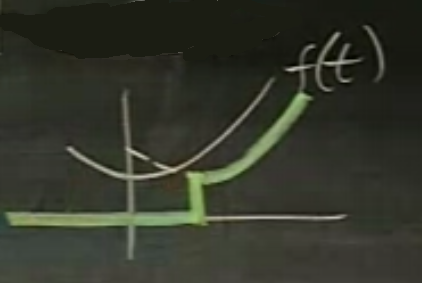
\includegraphics[height=2cm]{22_8.png}

\[ u(t-a)f(t-a) \leadsto e^{-as}F(s) 
\ \ \ \label{2}
\]

(2) gecisi Laplace Tablosunda gorulebilir.

Fakat $f$ cogunlukla $t-a$ formunda gelmez, mesela $\sin(t)$, $\cos(t)$
olur, o zaman su teknigi kullanabilirsiniz

\[ u(t-a)f(t) \leadsto e^{-as}\mathcal{L}(f(t+a)) \]

Bu teknige bazilari ustel kaydirma fonksiyonu (exponential shift formula)
diyor. Biz bu terimi kullanmayacagiz. Biz $t$ ekseni tercumesi (t-axis
translation) formulu diyecegiz. 

(2)'nin ispati

\[ \int_{0}^{\infty}e^{-st}u(t-a)f(t-a) dt \]

Ama formulde $F(s)$ kullanmak istiyorum, o zaman $f(t-a)$'yi bir sekilde
$f(t)$ yapmam lazim. Degisken degisimi yaparim. 

\[ t_1 = t-a \]

\[ = \int_{a}^{\infty}e^{-s(t_1+a)}u(t_1)f(t_1) dt_1 \]

\[ = e^{-sa} \int_{-a}^{\infty}e^{-st_1}u(t_1)f(t_1) dt_1 \]

$u(t_1)$ $t_1<0$ icin sifir olduguna gore $-a,0$ arasini entegral alt
sinirindan atabiliriz, 

\[ = e^{-sa} \int_{0}^{\infty}e^{-st_1}f(t_1) dt_1 \]

$u(t_1)$'in kendisini niye attik? Cunku sifir sonrasi 1 degerinde zaten. 

``Ama $t$ degiskeni $t_1$ haline geldi, artik bu Laplace Transformu olmaz''
diye dusunenler olabilir. Fakat entegrasyonda kullanilan fonksiyonun illa
$t$ ismini tasimasi gerekmiyor, cunku o degisken bir yer tutucu (dummy)
sadece. Entegre edilen, sinirlar duzgunse, ustteki de bir Laplace
Transformudur.

Yani

\[ u(t-a)f(t-a) \leadsto e^{-as}\mathcal{L}(f(t)) \]

$t$ yerine $t+a$ gecirdim.

Eger $u(t-a)f(t)$ olsaydi?

\[ u(t-a)f(t-a+a) \leadsto e^{-as}\mathcal{L}(f(t+a))) \]

Ornek 

\[ u_{ab} = u(t-a) - u(t-b) \]

\[ \leadsto \frac{e^{-as}}{s} - \frac{e^{-bs}}{s} \]

Ornek

\[ u(t-1)t^2 \]

Transformu nedir? 

\[ \leadsto e^{-s}\mathcal{L}((t+1)^2) = 
e^{-s}\mathcal{L} (t^2+2t+1) =
e^{-s}(\frac{2}{s^3} + \frac{2}{s^2} + \frac{1}{s})
 \]

Bayagi kalabalik bir sonuc oldu, fakat transformunu aldigimizda elde edilen
yukaridaki fonksiyon da o kadar basit bir fonksiyon degil zaten; altta
yesil renkle isaretli 

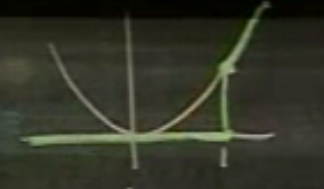
\includegraphics[height=2cm]{22_9.png}

Fonksiyon kesintili (discontinuous) bir fonksiyon. Kesintinin nerede
olustugu $e^{-as}$ formulunde $a$, yani $e^{-s} = e^{-1\cdot s}$ icin 1. 

* * *

\[ \mathcal{L}^{-1}\bigg( \frac{1+e^{-\pi s}}{s^2+1} \bigg) \]

Cevabin bir kesikli fonksiyon olacagini simdiden biliyoruz, cunku formul
icinde ustel bir fonksiyon var. Ilk yapacagimiz is ustel fonksiyonu yanliz
kalacak sekilde ifadeyi parcalamak. 

\[ = \frac{1}{s^2+1} + \frac{e^{-\pi s}}{s^2 + 1}\]

Once suna bakalim

\[ \frac{1}{s^2+1} \stackrel{-1}{\leadsto}  \ \ ? \]

Eger usttekine cevap olarak $sin(t)$ dersek, yanlis olur. Eger ustel
fonksiyon formulun geri kalaninda olmasaydi, o zaman $sin(t)$ olabilirdi,
ama simdi 

\[ \frac{1}{s^2+1} \stackrel{-1}{\leadsto} u(t)sin(t) \]

kullanmamiz lazim. Peki

\[ \frac{e^{-\pi s}}{s^2 + 1} \stackrel{-1}{\leadsto} \ \ ? \]

Yine (2)'yi kullanirim, 

\[\stackrel{-1}{\leadsto} u(t-\pi)sin(t-\pi) \]

Nihai cevap nedir? Iki parcayi toplarim

\[ \frac{1}{s^2+1} + \frac{e^{-\pi s}}{s^2 + 1} \stackrel{-1}{\leadsto} 
u(t)\sin(t) + u(t-\pi)\sin(t-\pi) 
\]

Bu cevap teknik olarak dogru, ama biraz masajlayip onu daha duzgun bir hale
getirmek lazim [hatta hoca sakayla karisik bu halde birakirsaniz sinavda
not kirarim diyor]. 

O zaman her parcaya teker teker bakalim. Formulun $u(t)\sin(t)$ kismi
sadece $t \ge 0$ icin anlamli, cunku ondan once birim step fonksiyonu
sifir. $u(t-\pi)\sin(t-\pi) $ kismi ise $t \ge \pi$ icin anlamli. Elimizde
iki tane senaryo var aslinda, o zaman bu fonksiyonu parcali, senaryolu
olarak gosterebiliriz. 

\[ 
f(t) = 
\left\{ \begin{array}{ll}
sin(t) & 0 \le t \le \pi \\
sin(t) + (-sin(t)) & t \ge \pi
\end{array} \right.
 \]

Terim $-sin(t)$, $sin(t-\pi)$'dan geldi, cunku $sin$'i $\pi$ kadar yana
kaydirirsak (altta kesik cizgili) 

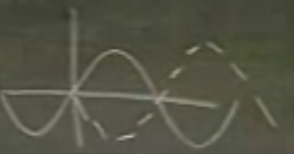
\includegraphics[height=2cm]{22_10.png}

elde edilen $-sin(t)$'dir. Nihai formul

\[ 
f(t) = 
\left\{ \begin{array}{ll}
sin(t) & 0 \le t \le \pi \\
0 & t \ge \pi
\end{array} \right.
 \]



\end{document}
